\def\year{2022}\relax
%File: formatting-instructions-latex-2022.tex
%release 2022.1
\documentclass[letterpaper]{article} % DO NOT CHANGE THIS
\usepackage{aaai22}  % DO NOT CHANGE THIS
\usepackage{times}  % DO NOT CHANGE THIS
\usepackage{helvet}  % DO NOT CHANGE THIS
\usepackage{courier}  % DO NOT CHANGE THIS
\usepackage[hyphens]{url}  % DO NOT CHANGE THIS
\usepackage{graphicx} % DO NOT CHANGE THIS
\urlstyle{rm} % DO NOT CHANGE THIS
\def\UrlFont{\rm}  % DO NOT CHANGE THIS
\usepackage{natbib}  % DO NOT CHANGE THIS AND DO NOT ADD ANY OPTIONS TO IT
\usepackage{caption} % DO NOT CHANGE THIS AND DO NOT ADD ANY OPTIONS TO IT
\DeclareCaptionStyle{ruled}{labelfont=normalfont,labelsep=colon,strut=off} % DO NOT CHANGE THIS
\frenchspacing  % DO NOT CHANGE THIS
\setlength{\pdfpagewidth}{8.5in}  % DO NOT CHANGE THIS
\setlength{\pdfpageheight}{11in}  % DO NOT CHANGE THIS
%
% These are recommended to typeset algorithms but not required. See the subsubsection on algorithms. Remove them if you don't have algorithms in your paper.
\usepackage{algorithm}
\usepackage{algpseudocode}
\usepackage{amssymb}
\usepackage{amsmath}

\newtheorem{theorem}{Theorem}
\newtheorem{definition}{Definition}
\newtheorem{lemma}{Lemma}

%
% These are are recommended to typeset listings but not required. See the subsubsection on listing. Remove this block if you don't have listings in your paper.
\usepackage{newfloat}
\usepackage{listings}
\lstset{%
	basicstyle={\footnotesize\ttfamily},% footnotesize acceptable for monospace
	numbers=left,numberstyle=\footnotesize,xleftmargin=2em,% show line numbers, remove this entire line if you don't want the numbers.
	aboveskip=0pt,belowskip=0pt,%
	showstringspaces=false,tabsize=2,breaklines=true}
\floatstyle{ruled}
\newfloat{listing}{tb}{lst}{}
\floatname{listing}{Listing}
%
%\nocopyright
%
% PDF Info Is REQUIRED.
% For /Title, write your title in Mixed Case.
% Don't use accents or commands. Retain the parentheses.
% For /Author, add all authors within the parentheses,
% separated by commas. No accents, special characters
% or commands are allowed.
% Keep the /TemplateVersion tag as is
\pdfinfo{
/Title (Towards a robot partner reducing ambiguities using perspective taking)
/Author (Anthony Favier, Shashank Shekhar, Rachid Alami)
/TemplateVersion (2022.1)
}

% DISALLOWED PACKAGES
% \usepackage{authblk} -- This package is specifically forbidden
% \usepackage{balance} -- This package is specifically forbidden
% \usepackage{color (if used in text)
% \usepackage{CJK} -- This package is specifically forbidden
% \usepackage{float} -- This package is specifically forbidden
% \usepackage{flushend} -- This package is specifically forbidden
% \usepackage{fontenc} -- This package is specifically forbidden
% \usepackage{fullpage} -- This package is specifically forbidden
% \usepackage{geometry} -- This package is specifically forbidden
% \usepackage{grffile} -- This package is specifically forbidden
% \usepackage{hyperref} -- This package is specifically forbidden
% \usepackage{navigator} -- This package is specifically forbidden
% (or any other package that embeds links such as navigator or hyperref)
% \indentfirst} -- This package is specifically forbidden
% \layout} -- This package is specifically forbidden
% \multicol} -- This package is specifically forbidden
% \nameref} -- This package is specifically forbidden
% \usepackage{savetrees} -- This package is specifically forbidden
% \usepackage{setspace} -- This package is specifically forbidden
% \usepackage{stfloats} -- This package is specifically forbidden
% \usepackage{tabu} -- This package is specifically forbidden
% \usepackage{titlesec} -- This package is specifically forbidden
% \usepackage{tocbibind} -- This package is specifically forbidden
% \usepackage{ulem} -- This package is specifically forbidden
% \usepackage{wrapfig} -- This package is specifically forbidden
% DISALLOWED COMMANDS
% \nocopyright -- Your paper will not be published if you use this command
% \addtolength -- This command may not be used
% \balance -- This command may not be used
% \baselinestretch -- Your paper will not be published if you use this command
% \clearpage -- No page breaks of any kind may be used for the final version of your paper
% \columnsep -- This command may not be used
% \newpage -- No page breaks of any kind may be used for the final version of your paper
% \pagebreak -- No page breaks of any kind may be used for the final version of your paperr
% \pagestyle -- This command may not be used
% \tiny -- This is not an acceptable font size.
% \vspace{- -- No negative value may be used in proximity of a caption, figure, table, section, subsection, subsubsection, or reference
% \vskip{- -- No negative value may be used to alter spacing above or below a caption, figure, table, section, subsection, subsubsection, or reference

\setcounter{secnumdepth}{0} %May be changed to 1 or 2 if section numbers are desired.

% The file aaai22.sty is the style file for AAAI Press
% proceedings, working notes, and technical reports.
%

% Title

% Your title must be in mixed case, not sentence case.
% That means all verbs (including short verbs like be, is, using,and go),
% nouns, adverbs, adjectives should be capitalized, including both words in hyphenated terms, while
% articles, conjunctions, and prepositions are lower case unless they
% directly follow a colon or long dash
\title
{
% old-1. Human-Aware Planning with Communication: \\ While Keeping Itself in Human's Shoes a Robot Plans for Both 
% Perspective Taking and Its Use for Communication in Planning: 
Planning with Communication Empowered by Situation Assessment:
\\ 
A Robot Builds Collaborative Plans
while Keeping Itself in Human's Shoes 
%While Keeping Itself in Human's Shoes a Robot Produce Collaborative Plans 
%is in Human's Shoes   
% old-2. Towards a robot partner reducing\\ ambiguities using perspective taking
}
\author{
    %Authors
    % All authors must be in the same font size and format.
    Anthony Favier\textsuperscript{\rm 1,2},
    Shashank Shekhar\textsuperscript{\rm 1},
    Rachid Alami\textsuperscript{\rm 1,2}
}
\affiliations{
    %Afiliations
    \textsuperscript{\rm 1}LAAS-CNRS, Universite de Toulouse, CNRS, Toulouse, France\\
    \textsuperscript{\rm 2}{Artificial and Natural Intelligence Toulouse Institute (ANITI)}

    % email address must be in roman text type, not monospace or sans serif
    \{anthony.favier, sshekhar, rachid.alami\}@laas.fr
}

\begin{document}

%%%%% SYMBOLS DEFINITION %%%%%
\newcommand{\worldstates}{\mathcal{S}}
\newcommand{\worldstate}{s}
\newcommand{\fluent}[3]{\mathcal{F}^{#1#2}_{#3}}
\newcommand{\prop}{\varphi}
\newcommand{\allprops}{\Phi}
\newcommand{\predicate}{\mathcal{P}}
\newcommand{\predval}{v}
\newcommand{\agent}{\lambda}
\newcommand{\beliefs}{\mathcal{B}}
\newcommand{\human}{H}
\newcommand{\robot}{R}
\newcommand{\places}{\mathcal{P}}
\newcommand{\place}{p}
\newcommand{\unknown}{UnKw}
\newcommand{\known}{Kw}
\newcommand{\missedactions}{\mathcal{M}}
\newcommand{\loc}[1]{loc(#1)}
\newcommand{\obs}[1]{obs(#1)}
\newcommand{\dom}[1]{dom(#1)}
\newcommand{\observable}{\texttt{OBS}}
\newcommand{\inferrable}{\texttt{INF}}
%%%%%%%%%%%%%%%%%%%%%%%%%%%%%%

\maketitle

\begin{abstract}
We consider the human-aware task planning (HATP) problem when a human-robot team is given a joint-task or joint-goal with a fully known task objective. 
The best current solver tackles such HATP problems by the robot performing collaborative, centralized planning while assuming itself and its human partner as one meta-agent. 
Moreover, the robot considers that a human cannot be supervised during plan execution like an artificial agent. And hence, to cater to that, during the planning phase itself, it emulates and predicts humans' actions, decisions, and reactions. 
To improve this solver, we describe a new planning approach that models and uses a novel run-time {\em observability} criteria enabled by existing concepts for situation assessment, and captures relevant agent's belief divergence that could arise in practice. 
% during planning. 
This approach effectively uses communication effectively, and decides ``if'' and ``when'' belief alignment is required during planning. 
These changes improve the planner's overall performance such that the planner uses communication optimally, and make the new method robust for more challenging real-world situations.  
\end{abstract}

\section{Introduction}
With the increasing penetration of sensor networks, advancements in robotic technology, the Internet of Things (IoT), etc., multi-robot systems are becoming ubiquitous, and the complexity of the tasks these autonomous robots can handle individually or together as a team is constantly increasing.
However, robots collaborating and (or) interacting with humans, for example, a robot hands-over, a robot achieving a joint-task with the help of a human or receiving some routine help from a human, etc., is seldom seen in our day-to-day life, but will soon become ubiquitous, too.

Consider a scenario in which you (a \textit{human} agent) want to prepare, together with your robot, some pasta in your kitchen. This joint task comprises several components and activities. For example, pasta packets are kept in the cupboard either in the kitchen area or the living room, lidding a pot, turning a furnace on, salt, spices, adding salt to the pasta, etc. 
Sometimes the needed objects to prepare pasta might be accessible only to you (or the robot) from your (its) current position, while some are accessible to both of you. 
Like this subclass of collaborative tasks, its multiple instantiations across many other real-world domains exist, e.g., homes, offices, hospitals, etc.

Naturally, the human would want to work alongside the robot but without being bothered too much and too often, or sometimes they are too lazy to perform an action assuming that the robot will do it instead, even if it takes longer to achieve the overall joint-task. 
% The human agent may \textit{choose} to leave the place during the task execution. Although, in these cases, the human agent is considered a fully cooperative and rational partner, they cannot be managed like an artificial agent (a fully controllable agent). But, the robot can always influence her behavior. 
% by eliciting her actions and emulating her mental state
In the cases that interest us, the human agent is considered a fully cooperative and rational partner but cannot be managed like an artificial agent (a \textit{fully} controllable agent). When the human agent has several ways to achieve a goal, the robot cannot control which way the human will choose.  However, the robot can still decide to act to influence human choices, and thus it elicits their actions. 

%Even 
It motivates us to consider one crucial aspect of human-robot collaborative planning: A robot should not only plan for human-robot joint (collaborative) actions but also predict and emulate human decisions and actions (and sometimes their reactions) to seamlessly achieve the task together. 
The robot must put itself in the shoes of the human agent, helping the robot to \textit{prohibit} the human agent executing an action with a detrimental effect on the overall joint-task achievement, e.g., this action ends up consuming some resource essential to achieving the task. 
Moreover, it also helps the robot to create a situation that will \textit{promote} an action to be executed by the human agent and is ``relevant'' to achieving the joint-task.       
% In this setting, it is common to compute a policy for all agents using a central engine. This policy is executed by
% the agents in a decentralized manner, and agent communication
% is performed through explicit actions.


% Considering these above scenarios: 
% There has been a series of 
Work on human task modelling and human-aware task planning to build a task planner focusing on human-robot collaboration and (\textit{partially}) dealing with issues we discussed earlier~\cite{alami2006toward,montreuil2007planning,alili2009planning,lallement2014hatp,de2015hatp,lallement2018hatp}.
%3684211}, unlike the previous approaches, the authors propose a more
Recently, in~\cite{BuisanA21,buisan:hal-03684211}, unlike the previous approaches, the authors propose a more suitable framework for these sub-class of HRI problems, which is comprising a \textit{dual} HTNs (Hierarchical Task Networks~\cite{naubooks0014222}) joint-task specification model: One model is for the human agent, and the other is for the robot. 
They assume that a domain modeler with expertise in robotics, human-human collaboration, human psychology, etc., is available to describe HTN specifications for such collaborative planning paradigms. 
The dual HTNs describe their individual capabilities, initial beliefs, shared tasks (goals), world dynamics, common ground or their understanding of the world, etc. Moreover, the modeler also implicitly describes \textit{hypothetical} variables, to capture a human's mood, intentions, etc., and they are not trivial to manage. 
Both these models are with the robot, while the robot plans for their actions based on these joint specification models, and predicts and emulates human actions, decisions, and reactions.    

HATP-EHDA is the state of the art planner~\cite{buisan:hal-03684211}, 
% Without loss of generality, it assumes that agents \textit{decide} to act (e.g., pushing a heavy box, moving, noop, idle, etc.) one after the other. 
generates a policy tree comprising human and robot actions. 
% Note that a 
The human is an uncontrollable agent,
% , so even if they are rational and collaborative, 
so it is hard to determine their ``next'' action upfront, which captures the impact of their mood or intention.
Therefore, for a sound execution, after every robot action, the policy tree gets branched on all possible \text{choices} available to the human.

The planner makes some unrealistic assumptions. For example, an action performed by one agent would also impact the beliefs of other agents, i.e. it implicitly considers that those other agents always observe this agent acting and share the same perspective as this agent. However, in reality, a robot can act that can impact human's belief differently under different scenarios. For example, activities like the robot adding some salt to the pasta, or turning on the furnace, would impact the human's belief differently depending on whether the human is available in the kitchen at the time of action execution.   

% HATP-EHDA assumes that if the robot executes an action, the human's belief gets updated, along with the robot's belief, or vice versa. It means that all the action execution is observable to both these agents. It is a \textit{major} drawback of the solver, since it is not always the case in reality. For example, in the pasta preparation scenario, suppose the human leaves the kitchen, and before they arrive back in the kitchen, the robot \textit{adds} some salt to the pasta, \textit{lids} the pot, and \textit{turns} on the furnace. 
% Later, when the human arrives in the kitchen: What would be the new belief of the human? Certainly, they will observe that the furnace is {\sc on}, and also the pot is closed. But what about ``there is already some salt in pasta?'' Which creates divergence in the agents' belief states. 
% % In such scenarios, 
% To simplify the reasoning process over multiple task models, we assume that the robot is always aware of the ground truth. That means we ignore the uncertainty associated with what the human does when the robot is absent. 
% And any advancement in this direction is left for future work. 

% In principle, HATP-EHDA can model and specify all the cases with some (ungraceful) modifications at the model specification level, which may arise in human-robot collaborative planning. (The related work section discusses this in detail.)

% can handle different initial distinct beliefs
% To make it more realistic, 
We introduce a novel paradigm for {\em execution time observability} in the HATP-EHDA framework --- thanks to existing situation  assessment reasoners which perform spatial reasoning and perspective taking ~\cite{flavell1992perspectives,trafton2005enabling,johnson2005perceptual,Sisbot2011SituationAF}, and propose a new planning approach 
% (based on
% by extending and 
% improving 
% HATP-EHDA) 
to handle divergences in human-robot individual beliefs about the ground truth.
%23dito
Our approach models explicit communication actions, and to tackle belief divergence effectively while planning with communication actions.
% To do so, 

% We extend the HATP-EHDA framework. 
% We thank the modeler again for explicitly specifying, which state variables/fluents are \textit{observable} (an persistent effect of an action, e.g., turning on the furnace, which the human can observe with the help of \textit{situation assessment} (SA)~\cite{cite?} -- SA helps the human to assess the environment), \textit{inferrable} -- an effect of an action being executed by some other agent, which can only be inferred when the agent sees the action being performed by the other agent, e.g., robot adding some salt to the pasta and human sees it doing so. 
% The latter can be informed about the exact value of the inferrable state variables, otherwise, to manage the belief alignment.   
%- both human and robot beliefs will be updated 

% Communication paradigms like text, visual, speech, etc., are prerequisites for building a communication protocol among multiple agents. However, 
Effective use of a communication modality is essential to achieve the motivation behind their development, say, a seamless collaboration. However, in reality communication incurs some costs. 
While in many human-robot interaction (HRI) scenarios, communicating too much or too little can hamper or delay the overall task achievement process. 
Therefore, deciding ``How to communicate?'' is crucial, but it is equally significant to decide ``If, When, and What to Communicate?'' 
We assume that a natural language-based speech modality is available, while 
% if, when, and what to 
% whether to communicate 
the decision about communication is made by the new algorithm. 
% with communication actions.
%

The paper is structured as follows: We first build a relevant background to understand this framework and discuss the related work. We then discuss the methodology: which includes modeling and planning with communication actions. 
After that, we present the results and show examples where handling the belief divergences is effective and how HATP-EHDA is ineffective under those scenarios. We compare the overall effectiveness of our approach and prove that it does not use communication more than needed (avoids verbosity) in the process. We conclude with a summary, discussion, and future work.

\section{Background}
% In this section, we build a relevant background, providing some essential definitions and discussing problem models and planning frameworks on which this work is based.

Some generalized basic terminologies related to HTNs are presented, e.g. the model, problem definition, and its solution~\cite{naubooks0014222}.  
\begin{definition} 
(\textbf{Task Network}.) {A task network is a 2-tuple $w=(U,C)$, where $u\in U$ is a task node, while $t_u$ is the task associated to this node. $C$ is the set of constrains - includes strict (partial) orderings between task nodes, variable binding constraints, etc. If $\forall u \in U$, $t_u$ is a primitive task, the task network is primitive; otherwise it is non-primitive.}  
\end{definition}

\begin{definition}
\textbf{(HTN Planning Problem.)} 
The HTN planning
problem is a 3-tuple $\mathcal{P} = (s_0, w_0, D)$ where $s_0$ is the initial belief state (the ground truth), $t_0$ is the initial task network, and $D$ is the HTN planning domain which consists of a set of tasks and methods.
\end{definition}
A domain is a 2-tuple $D=(O, M)$ where $O$ is the set of operators and $M$ is the set of methods. An operator $o \in O$ is a primitive task described as $o=(name(o), pre(o), \textit{eff}(o))$, which correspond to operator name, its precondition, and its effect, respectively. 

A \textit{task} consists of a task symbol and a list of parameters. It is called a \textit{primitive} task if its task symbol is an operator name and its parameters match, otherwise it is a \textit{non-primitive} task. This also means that we know how to execute a primitive task, while to execute a non-primitive task, we need to decompose it to sub-tasks using \textit{methods}. 

A method ($m \in M$) is a 4-tuple $m=(name(m),task(m),subtasks(m),constr(m))$ which are name of the method, a non-primitive task, a set of sub-tasks, and a set of constraints, respectively. $m$ is relevant for a task $t$ if there exists a parameter substitution $\sigma$ such that $\sigma(t) = task(m)$. Note that there could be different methods relevant for a single task $t$, decomposing this task differently. $(subtasks(m),constr(m))$ is a task network.      

Suppose $m$ is an instantiated method, and $task(m)=t_u$ then $m$ decomposes $u$ into $subtasks(m')$, producing a new task network, $\delta(w,u,m)=((U-\{u\})\cup subtasks(m'),C'\cup constr(m'))$.
Here, every \textit{precedence}, \textit{before} constraints, \textit{after} constraints, and between constraints between tasks are carefully maintained (after each decomposition).

\begin{definition} 
(\textbf{Solution Plan}.) 
{A sequence of primitive actions $\pi=(o_1,o_2,o_3...,o_k)$ is a solution plan for the HTN planning problem $\mathcal{P}=(s_0,w_0,D)$ iff there exists a primitive decomposition $w_p$ (of the initial task network $w_0$), and $\pi$ is an instance of it. 
}  
\end{definition}

We now shift the discussion to HATP-EHDA -- a framework comprising a dual-HTNs task specification model.   
For ease of exposition we consider a team of a single human and a single robot. Two categories: The robot HTN model $\mathrm{HTN}_{r}$, represents the task specifications for a controllable agent, while $\mathrm{HTN}_{h}$ represents the HTN model for the human partner, who is an uncontrollable one but the planner has a
representation of their decision, action, and reaction models. 
% Hierarchical modeling of human-centred activities has been exploited in human-computer interaction in the literature~\cite{annett1967task,paterno2004concurtasktrees,martinie2019analysing}.

% ut loss of generality, only one agent
Note that we discuss only a high-level, general framework here and minor details are purposely skipped due to the page limit constraint. More details on this are provided in~\cite{thesisBuisan21,buisan:hal-03684211}. 

In the interest of this work: The agents start with a joint task network, means they have a shared $w_0$ to start with in their respective task models: $\mathrm{HTN}_{h}$ and $\mathrm{HTN}_{r}$. The new problem, $\mathcal{P}_{hr}$, composed of these two networks. Decomposing a non-primitive task, updating the current network with new constraints, etc., are generalized accordingly for the \textit{two-agent} scenario. 

Without loss of generality, the solver assumes that only one agent acts at a time, while also, one agent acts after the other in planning and execution. 
We do not add any further information in the individual task models during plan elaboration. It means, we start with building the whole search-space by considering all possible feasible decomposition. Later, we use/adapt off-the-shelf graph-search algorithms (e.g., $A^*$, $AO^*$, etc.) and use social cost, plan legibility and acceptability, etc., for the search process to extract a \textit{joint solution plan} for both the human and the robot. 

\begin{definition}
(\textbf{Joint Solution Plan}.) 
{It is a solution for $\mathcal{P}_{hr}$, represented as a tree or a graph, i.e., $G=(V,E)$. Each vertex ($v \in V$) represents the robot's belief state, starting from the root node $s_0^r$. Each edge ($e \in E$) represents a primitive action that is either a robot's action $o^{r}$ or a human's action $o^{h}$. $G$ gets branched on the possible choices ($o^{h}_1$, $o^{h}_2$, ..., $o^{h}_k$). 
% available for the human in the given state and its human's turn to act next.
}  
\end{definition}

The requirement from this solution tree is that for each branch, from the root to a leaf node, the sequence of primitive actions, say,  $\pi=(o_1^r,o_2^h,o_3^r,...,o_{k-1}^h,o_k^r)$ is a solution plan for the HATP problem, $\mathcal{P}_{hr}$. Here, each $o_i^h$ represents a choice the human could make (out of several) during execution.
% , which means there exists a primitive decomposition $w_p_{hr}$ of the initial joint-task network $w_0$, and $\pi$ is an instance of it. 

\paragraph{Situation Assessment} In human psychology, especially in human-human interaction, spatial reasoning and perspective taking is crucial. 
Using an existing approach from the literature, we can form relations between objects and (artificial) agents or objects and their environment to have natural human-robot collaboration, the way they have been used to gather the knowledge and capabilities of people around us. 

In this work, we use existing technology in HATP-EHDA to access the environment, such that the robot keeps itself in human's shoes to predict and emulate human's knowledge and behavior. Currently, the robot's belief is assumed to be the ground truth. But the human's perspective and belief about the world may differ depending on whether she was present when the robot acted. Moreover, it is possible when some object is hidden for the human but is available for the robot even if the agents are co-present. Thanks to situation assessment, we can now define and plan with execution time observability criteria in a principled way. We can keep an account on agents' belief divergence that may occur in practice due to spatial reasoning and perspective taking. 

\subsection{Related Work}
A robot acting in an environment in the presence of a human needs to consider the evident constraints, e.g., plan pertinence and acceptance of its activities by the human while considering their course of joint-actions.
Most proposed approaches based on hierarchical task decomposition concepts to human-aware collaborative task planning assume a fully controllable and cooperative human that is willing to participate in achieving a joint-goal~\cite{sebastiani2017dealing,alami2006toward,lallement2014hatp,lallement2018hatp}.

\textbf{(This section is NOT finished!! Will work next week.)}

\section{Execution-Time Observability Conventions}
At a high-level, the formalization below is based on the standard state-variable representation (we refer the reader to~\cite{naubooks0014222}) with some minor abuse of the standard notations to maintain the flow of the discussion.

To describe an environment a set of \textit{constant symbols} is used. Usually, these constants are classified in different groups ($gr$), e.g., places, pots, agents, etc. 
Each constant can be represented as an \textit{object symbol}, e.g., \textit{robot1}, \textit{human2}, \textit{pasta-pkt1}, etc. 
An \textit{object variable} belonging to a group can be \textit{instantiated} using any constant symbol of that group.

Suppose $\mathcal{S}$ is the complete state-space and $s \in \mathcal{S}$ represents a single state (or a \textit{belief state} in the current context).  

% We start with some basic definitions below:

\begin{definition}
\textbf{(State Variable Function.)} It is represented as: $f_{sym}:(?g_1 (gr_1), ?g_2 (gr_2), ..., ?g_k (gr_k),\mathcal{S})\rightarrow ?g_{k+1} (gr_{k+1})$. 
\end{definition}
Here, $sym$ is \textit{state-variable symbol}, while each \textit{term} with a notation $?$, can be instantiated with a constant symbol from its respective \textit{group} mentioned inside $()$ right besides the term. 
For example, to model agents' location in a state, we use $f_{AgtAt}:(?a (Agents), \mathcal{S}) \rightarrow ?r (Rooms)$, representing, for each agent and each possible, an a given legal state ($s_i \in \mathcal{S}$), we know where the agent is located in $s_i$. 
Each such possible \textit{instantiation} of defined state variable functions, represents $s_i$ partially, and it is also called as a characteristic attribute of $s_i$.     
 
Suppose $s \in \mathcal{S}$ is the real state. As per our assumptions, the belief state of the robot is always the real world state, i.e., $B_{\varphi_r} = s$, and the human belief is $B_{\varphi_h}$ -- that is generated when the robot takes the human's perspective. Each state variable function instantiation with respect to a belief state, $B_{\varphi_r}$ ($B_{\varphi_h}$), represents the truth value of that state attribute with the \textit{perspective} of that agent, $\varphi_r$ ($\varphi_h$). (Both perspectives are managed by the robot in the setting of our interests.) 

\begin{definition}
\textbf{(Belief Divergence.)}
Suppose that $f_{\textit{svs}}:(g_{(1)1},g_{(2)1},...,g_{(k)1},s)\rightarrow g_{(k+1)1}$, for a given legal current state $s$, is a possible {\em grounding} of a state-variable function with the function symbol $\text{\em svs}$. 
If there exists an instantiation such that $f_{\textit{svs}}:(g_{(1)1},g_{(2)1},...,g_{(k)1},B_{\varphi_r}) = {g_{(k+1)1}}  \neq f_{\textit{svs}}:(g_{(1)1},g_{(2)1},...,g_{(k)1},B_{\varphi_h})$, then the human belief diverges.  
\end{definition} 
% Consequently, belief divergence is caught.
Note that both the agents are always definite about their individual knowledge of the current state. (In this case, unless the human somehow learns the truth.)

\begin{definition}
\textbf{(Places.)} Represent a group of constants such that each member of this group captures some area in the environment defined by the modeler apriori.  
\end{definition}
Two agents present at a place simultaneously are said to be co-present or co-located.

We associate each attribute (a fully grounded state-variable function) of a state to a place. For example, if the robot turns on the furnace placed in the kitchen, then $f_{\textit{TurnOn}}(\textit{furnace}, s, kitchen) \rightarrow \textit{boolVal}$ such that $\textit{boolVal} \in \{\textit{true},\textit{false}\}$ and only for the constant $kitchen$ it takes \textit{true} for all other object variable from \textit{Places}, the state variable function returns \textit{false}. We note that our current planning system is unable to do this type of reasoning, and hence we take a liberty here to manage it manually so that the main contribution can be targeted. 
Similarly, action schema is managed as state attributes are also a part of precondition and effect of an action. 

\begin{definition}
\textbf{NEW (Location function.)}
Each \textit{state-variable symbol} is associated to a place through a location function $loc(f_{\textit{svs}}, s) \rightarrow \place \in \places$.
\end{definition}
These relations help to describe the world state by expressing where the state-variables are effective and observable. Currently, the locations has to be updated manually in the action's effects.

\begin{definition}
\textbf{(Observability type function.) (ref to Obesrvability of fluents section)}
The observability type of each \textit{state-varibale symbol} is defined by the function $obs(f_{\textit{svs}}, s) \rightarrow o \in\{\observable, \inferable\}$.
\end{definition}
For now, we assume the observability types are constant and initially defined.

Explanation $\observable$ and $\inferable$.


\textbf{****************************}

\textbf{**** }

\textbf{**** }

\textbf{unpolished text below}

\textbf{**** }

\textbf{**** }
% 

% what is known ? our understanding of the world
General context, towards robot partner. 

% what is unknown ? the gap we want to fill
% how and why ? your rational and purpose/hypothesis 

\textbf{Choice to reduce ambiguities [example, as introduction]}:
Let's assume the human and the robot have to cook together and at some point salt needs to be added to a dish. The robot adds salt to the dish while the human is away. When coming back, the human has no way to know if there is salt just by looking at the dish.
Then three cases can occur : 1) The human considers that the robot didn't add salt, thus they will to add more, 2) The human considers that the robot added salt, so the goal is reached, 3) the human prefers to directly ask the robot if it added salt. 
Humans are rational, so they will rarely blindly act without at least asking the state of the shared plan. However, whatever case we are in, an ambiguity will remain for the human, and we are able to predict it. Thus, we decide to proactively reduce the ambiguity by communicating about their belief divergences or the missed actions. This communication might seem optional in some situations but having a plan without ambiguities in the context of a shared goal is often much better than a plan with fewer steps but where agent aren't sure about what they have to do.

% \clearpage
\section{Related Work}

\begin{itemize}
    \item Some refs from ICRA paper ? (Devin theory of mind) 
    \item Human activity model, hierarchical HTN
    \item HATP general
    \item HATPEHDA (ICRA)
    \item explicit communication, multi agent 
    \item belief divergences, non verbal com
\end{itemize}

\section{Background}
HATPEHDA concept and definitions

The work \cite{buisan:hal-03684211} already support collaborative task planning while maintaining distinct beliefs/knowledge for each agent. This work is itself an extension of HATP \cite{hatp?} having one search thread for a shared plan resulting in two coordinated plan streams. The last work HATPEHDA proposes a two threads search. Based on this work, we enhanced the task planner with a few concept linked to perspective taking and observability in order to reduce the ambiguities that may happen in a collaborative task. First we predict the situation assessment of an agent. On the other hand, we look for belief divergences that have a detrimental influence on the plan in order to fix them with communication. We also check observability of action execution to update beliefs with different types of effects.

Agents can have a shared goal but no shared plan. There is no plan negotiation between the agents, so the robot is only able to estimate what the human will do and plan its own actions according to that.

\subsection{HATPEHDA background/basis and definitions}

The main structure manipulated by our planner is the \textbf{agent}, more precisely two will be represented, the \textit{human} and the \textit{robot}. Each agent has their own \textbf{beliefs}, \textbf{action model}, \textbf{agenda}, \textbf{plan} and \textbf{triggers}. The planner has to use their action models and beliefs to decompose the tasks in their agenda into primitive tasks (actions) that are inserted in their plan. By doing so, it also has to update the beliefs of each agent and to model their reaction by executing the triggers. \cite{buisan:hal-03684211}.

The agents, robot and human, have each a distinct action model modeled with HTNs. The robot HTN starts with the goal given to the robot and describes how to decompose that abstract goal into several actions. The human HTN represents the anticipation by the robot of the human plan and possible actions in a given situation. Other formalism like POMDP or PDDL could be used to describe the agents' action models as soon as they provide the next possible actions of an agent in a given state. Especially the human one which is an estimation.

The planner has a goal creation mechanism, especially for the human, based on goal-directed or situation-directed task creation.

The planning algorithm is implemented as a search involving two threads: 1) the robot task-based plan search using the robot action model 2) the estimation of the human task-based plan search using the human action model.

While HTN-R corresponds to the controllable part  (from the robot point of view) of the (shared) plan, HTN-H represents the contingent part of the plan: the decisions and actions of the human. 

Hence, the obtained plan has two streams (one for the human and one of the robot) and is conditional. Alternatives correspond to human decision: choosing to act or not, making one (out of several choices).

As a result, HATP/EHDA allows to clearly separate what is planned for the robot and what the human can potentially do with respect to the task at hand. Besides, it allows to also:
\begin{itemize}
    \item deal with cases where the task is only given to the robot and not shared by the human
    \item manage the creation of a shared goal
    \item provide a mean to implement elicitation, by the robot, of decisions or reactions of the human
\end{itemize}
In our case the plan process starts:
\begin{itemize}
   \item with a goal given only to the robot: a task placed at the root of HTN-R (ex: Human asks the robot to achieve a goal)
   \item or with a shared goal: the same task is placed at the roots of  the two HTNs (ex: Human says to the robot: "Let us do X")
\end{itemize}

Situation-directed task creation in HTN-H allows to model (potential) reaction by the human to a situation created by after a given action of the robot. This can be used in the planner to elicit a reactiion of the human.

\textbf{HTN formalism [in background ?]}:
An HTN \textit{planning problem} is the 3-tuple $\langle d, S_0, \mathcal{D} \rangle$, where $d$ is the sequence of (primitive or abstract) tasks to solve, $S_0$ is an initial state as in classical planning, and $\mathcal{D}$ is an HTN \textit{planning domain}. Specifically, an HTN \textit{planning domain} is the pair $\mathcal{D}=\langle\mathcal{A},\mathcal{M}\rangle$ where $\mathcal{A}$-the primitives of the domain-is a finite set of operators as before, and $\mathcal{M}$ is a finite set of \textit{methods}. A \textit{method} is a tuple consisting of the name of the method, the abstract task that the method is used to solve, a precondition specifying when the method is applicable (like an operator's precondition), and a \textit{body} indicating which tasks are used to solve the task associated with the method. The method-body is a sequence of primitive and/or abstract tasks. 

The planning process works by selecting applicable reduction methods from $\mathcal{M}$ and applying them to abstract tasks in $d$ in a depth-first manner. In each iteration this will typically result in $d$ becoming a "more primitive" sequence of tasks. The process continues until $d$ has only primitive tasks left. At any stage in the planning process, if no applicable method can be found for an abstract task, the planner essentially "backtracks" and tries an alternative method for an abstract task refine earlier.

\textbf{Computing next possible agent actions / refining agenda [nothing new here, in hatpehda background ?]}:
% The refinement of the HTNs is mostly done thanks to the function $refineAgenda()$. This function keeps refining the agenda of an agent in a given state until reaching a not done primitive task at the first spot. It returns a refinement which is list of decomposition, one for each applicable methods. Each decomposition is a list of the obtained subtasks which starts with a not done primitive task. The second parameter the function $refineAgenda$ can be used to specify with which beliefs the refinement has to be done. 
The action model of each agent is described with a HTN. Thus, the process to compute (or estimate in the human case) the next possible actions of an agent is very close to classic HTN refinement.
The classic planning process for HTN planning problem consist in selecting applicable reduction methods from $\mathcal{M}$ and applying them to abstract tasks in $d$ in a depth-first manner. In our contribution the planning process slightly differs from the classic process since the goal is to compute or estimate all possible next actions in a given state. 
Here, $d$ corresponds to what we call the agenda of the agent. To compute the next possible actions the agent's agenda is refined. To do so the first task in the agenda is popped, and all applicable reduction methods are applied to the task resulting is search branches with different subtasks. The process is repeated for each created branch until reaching a primitive task in each of them. The primitive tasks from each search branch constitute the set of all possible next actions of the agent.
A search branch can refine into nothing but if all search branches refine into nothing then the first task popped from the agenda is done, so the next task in the agent's agenda is popped and refined. 
A search branch, corresponding to a list of subtasks, is called a decomposition. The list of all obtained decompositions is called a refinement.  


\section{Materials and Methods}
% what did you do ?



\subsection{Knowledge representation and observability definitions}

Our formalism is close to the SAS+ Formalism applied to HTN.(Probably to remove, might bring more confusions than explanations)

\textbf{Word state}: 
Let $\worldstates$ be the set of all possible world states. World states are defined by a same set of fluents. Each world state is fully described by the value of all its fluents at a given time i.e. $\forall\worldstate\in\worldstates, \worldstate=\{ \fluent{\worldstate}{}{} \}$.

\textbf{Fluent}: 
A fluent $\fluent{\worldstate}{}{}$ is a multi-valued state variable associated to a finite domain $\dom{\fluent{\worldstate}{}{}}$ partially describing the state of the world at a given time.

% (introduce loc ?)
% The observability type of fluents is qualified through the relation $\obs{ \fluent{\worldstate}{}{} } \in \{ \observable, \inferable \}$. 

e.g. Considering the following fluent $\fluent{\worldstate}{}{temp\_water}$, if initially the water is hot then $\fluent{\worldstate_0}{}{temp\_water}=hot$.

\textbf{Belief divergence}: 
We note $\fluent{\worldstate}{,\agent}{}$ a fluent evaluated in the perspective of an agent $\agent$. Thus, for a given real state of the world $\worldstate\in\worldstates$, the robot and the human can have different values for the same fluent. We call such mismatch a belief divergence.

e.g. $(\fluent{\worldstate_0}{,\robot}{temp\_water}{}=hot) \neq (\fluent{\worldstate_0}{,\human}{temp\_water}=cold)$

\textbf{Two distinct Beliefs}: 
We call beliefs of an agent $\agent$, noted $\beliefs_\agent$, the belief state in which this agent thinks the world is in, i.e. the set of all fluents evaluated in their perspective at a given time: $\beliefs_\agent=\{ \fluent{\worldstate}{,\agent}{} \}$. It is important to note that we use two distinct belief states during the planning process. On one hand, we consider the beliefs of the robot $\beliefs_\robot$ which are obtained through perception and effects of robot actions and decisions. And as we consider the planner as being part of the robot, we assume that $\beliefs_\robot$ is the ground truth estimation for the planner. On the other hand, we consider the human's belief state $\beliefs_\human$ which is only estimated by the robot by doing some perspective-taking reasoning during the planning process (and before ?).

\subsection{Place-based observability model}

We introduce a place-based model of observability. An agent observes and can only observe what happens in their current place, this includes action executions and fluent values.

\textbf{Places}: 
A place is an area defined a priori in the environment. Let $\places=\{ \place_i \}$ be the set of all defined places. Agents are always situated in a place or moving between them. Two agents situated in the same place are said to be co-present. Actions are always performed in a place. (Most?) State variables are associated to a place.

\textbf{Observation of an action execution}: 
The execution of an action performed by an agent $\agent$ is observed by all agents that were co-present with $\agent$ either before or after the action. The co-presence is checked both before and after to cover navigation actions.

\textbf{Observability of fluents}:
Each (most?) fluent is associated to a place $\place \in \places$ through the relation $\loc{ \fluent{\worldstate}{}{} }=\place$. These relations help to describe the world state by expressing where the fluents are effective and observable. (If $\loc{ \fluent{\worldstate}{}{} } = \varnothing $ then the fluent is ubiquitous). These relations can be dynamic for example when the fluent describes a property linked to a moving entity. Currently, the location of a fluent has to be updated manually in the domain if it is dynamic (we should go for an "entity-based" description of the world state to automatically update).

The observability type of each fluent is constant and defined initially through the relation $\obs{ \fluent{\worldstate}{}{} } \in \{ \observable, \inferable \}$. 
The first value $\observable$ means that the fluent is observable. A fluent is observed by an agent only if it is observable and if that agent is in the place associated to the fluent. 
Note that places can be symbolic and not only physical/geometric to represent more complex situation. For instance, let's consider the fluent $\fluent{\worldstate}{}{at\_o}$ describing the position of an object \textit{o}. The object is in the kitchen inside a cupboard that can either be open or closed. This situation can be modeled as follows :
\begin{itemize}
    \item $\fluent{\worldstate}{}{at\_o}=cupboard$
    \item $\obs{ \fluent{\worldstate}{}{at\_o} }=\observable$
    \item $\loc{ \fluent{\worldstate}{}{at\_o} } \in \{ kitchen, closed \}$
\end{itemize}
The relation $\loc{ \fluent{\worldstate}{}{at\_o} } = kitchen$ corresponds to when the cupboard is open, which means any agent in the place $kitchen$ can observe the object. On the other hand, when the cupboard is closed, $\loc{ \fluent{\worldstate}{}{at\_o} } = closed$, the agent cannot observe the object.

The other value $\inferable$ qualifies inferable fluents. A fluent is inferable if its value isn't observable but can be inferred by attending an action affecting that fluent. For instance, by observing someone adding salt to a dish we infer that there is now salt in the dish, although the salt in the dish isn't observable. It means that without attending the action execution it's impossible to tell if there salt just by looking at it. Thus, when an action affects inferable fluents only the co-present agents gets their beliefs updated. We later refer to actions affecting inferable fluents as actions with inferable effects (resp. with observable effects).


\subsection{Beliefs updates}

Agents' beliefs are updated by four different processes: 1) performing an action, 2) attending inferable effects, 3) assessing the situation, and 4) communicating about a relevant belief divergence.  

\textbf{Performing actions / Inferable effects}: 
When an agent performs an action its own beliefs are always directly updated with the action's effects.

The other agent's beliefs are updated about these effects through two mechanisms. The first one, that will handle observable effects, is the situation assessment and is detailed just after. 
The second one concerns inferable effects. As mentioned before, only agents that observed the action execution get their beliefs updated with the inferable effects.

For now, we assume that if we estimate that the human will perform a task not observable by the robot then it should remain quite simple like a series of deterministic actions. Basically, we currently do not handle more complex cases where the human has multiple choices of actions while not being observable. Considering this hypothesis, the robot beliefs are always updated with the effects of human actions, weither they are co-present or not.

\textbf{Situation Assessment}:
The idea is to predict the situation assessment of an agent and update their beliefs according to what they can see in their current place. When executed, each agent $\agent$ updates their beliefs with the ground truth value of every observed fluents, i.e. for every observable fluents ($\obs{ \fluent{\worldstate}{}{} } = \observable$) located in their place ($\loc{\fluent{\worldstate}{}{}} = \fluent{\worldstate}{}{at\_\agent}$), we have $\fluent{\worldstate}{,\agent}{} \gets \fluent{\worldstate}{}{}$. The situation assessment is executed after every action execution. This way, the agent's beliefs are updated either with the observable effects of an action performed by another co-present agent, or with the observable effects they missed when entering another place. 
Note that since the ground truth is actually the robot beliefs, this situation assessment is only effective for other agents, so here the human. 

\textbf{Relevant belief divergences checking}:
We want to detect if a belief divergence influences the plan of the human, i.e. if when using the human beliefs containing belief divergences induces different human actions than the ones expected using the ground truth beliefs. If so, the belief divergences are qualified as relevant. Indeed, a belief divergence can wrongly affect the applicability of a human action, its cost and its effects. 
Any difference in the human plan makes it either not applicable in reality, more expensive or with undesired effects. There are some rare cases of belief divergences inducing a different plan still applicable, with a similar cost and no undesired effects. But for now we omit those cases, and we consider relevant belief divergences as always detrimental. 
Note that there can be belief divergences not affecting the plan which will not be considered as detrimental.

To check if there are some relevant belief divergences we proceed as follows. When refining the human agenda to estimate their next possible actions, we first use the human beliefs $\beliefs_H$. The process is repeated but considering the robot beliefs $\beliefs_R$ (ground truth). The two obtained refinements are then compared to check if they are the same. Two refinements are considered to be the same if they respectively have the same decompositions, i.e. if, in both refinements, each decomposition respectively has the same type, subtasks and if their actions have the same applicability, cost and effects. 
If a difference is spotted we consider that there are relevant belief divergences to align, but we don't know which ones yet.

\textbf{Identify the relevant divergences and communicate}: 
Once the presence of relevant belief divergences has been confirmed they have to be identified. All divergences between $\mathcal{B}_R$ and $\mathcal{B}_H$ are first computed. Then the divergence's corrections are simulated one after another (i.e. $ \fluent{\worldstate}{,\human}{i} \gets \fluent{\worldstate}{,\robot}{i}$) and the human agenda is refined again in order to compare the new refinement with the one previously obtained with $\beliefs_\robot$. We keep simulating combination of divergence corrections in a breadth-first (search) manner until the refinements are the same, which means that all the relevant divergences have been identified. In the worst case, the two refinement are not the same until reaching the last combination which corresponds to all divergences being corrected, thus where $\beliefs_\human$ and $\beliefs_\robot$ are the same. So the obtained refinements will necessarily be the same which guarantees the ending of our algorithm. After having identified the divergences to correct in order to obtain the same refinements, the corresponding communication action is inserted in the robot's plan to inform the human about their relevant belief divergences and to correct them.
    
Communication actions are supposed to be instantaneous and able to correct several divergences at once. For now they are inserted right before the detected erroneous human action. (A more complex reasoning could be added to identify the optimal place to insert the communication action in the plan). 

% \textbf{Choice to reduce ambiguities}:
% In the case of a shared goal, let's assume that the human didn't observe the robot performing an action with only inferable effects, so when coming back the human has no way to tell if the action has been done just by looking at the scene. 
% Then three cases can occur : 1) The human considers that the robot didn't perform the action, thus the human will try to perform it again, 2) The human considers that the robot performed the action, so the plan execution continues, 3) the human prefers to directly ask the robot if it performed the action. 
% Humans are rational, so they will rarely blindly act without at least asking the state of the shared plan. However, whatever case we are in an ambiguity will remain for the human, and we are able to predict it. Thus, we decide to proactively reduce the ambiguity by communicating about their belief divergences or the missed actions. This communication might seem optional in some situations but having a plan without ambiguities in the context of a shared goal is often much better than a plan with fewer steps but where agent aren't sure about what they have to do. Communication help to compel the human actions.


\subsection{Algorithm (Optional maybe ...)}
MAYBE OPTINAL because it involves mechanisms not introduced (or maybe we should introduce them in the background ?) like the triggers and the WAIT/IDLE actions.

The refinement of the HTNs is mostly done thanks to the function $refineAgenda()$. This function keeps refining the agenda of an agent in a given state until reaching a not done primitive task at the first spot. It returns a refinement which is list of decomposition, one for each applicable methods. Each decomposition is a list of the obtained subtasks which starts with a not done primitive task. The second parameter the function $refineAgenda$ can be used to specify with which beliefs the refinement has to be done. 

The returned refinement in Alg.~\ref{alg:ap_ref_all} contains the subtasks obtained through the refinement of the agenda after a potential belief alignment, application of the actions, situation assessment and triggers.

\begin{algorithm}
\caption{Get applied refinement ALL}\label{alg:ap_ref_all}
\begin{algorithmic}
\Require $h\_name$: human name, $r\_name$: robot name, $ags$: all agents

\State $ref \gets refAgenda(ags, ag\_name)$

\State $ref\_r \gets refAgenda(ags, r\_name)$ \Comment{H only}
\If{$relevantDivergences(ref, ref\_r)$} \Comment{H only}
    \State $alignBeliefsWithComAction()$
    \State $ref \gets refAgenda(aligned\_ags, h\_name)$
\EndIf

\For{$decomp$ in $refinement$}

    \State $result \gets applyOperator(dec, ag\_name)$ 
    \If{$notApplicable(result)$}
        \State \texttt{add wait, idle or end}
    \Else
        \State $applyOperator(dec, r\_name)$ \Comment{H only}
        \State $applyInferableEff(dec, h\_name)$ \Comment{R only}
        \State $humanSituationAssessment()$
        \State $checkTriggers()$
        \State $updateDecomp(decomp)$
    \EndIf
\EndFor

\State \Return ref

\end{algorithmic}
\end{algorithm}



\section{Results}
% what results did you get ?


Explicitly say that previous version of hatpehda do not handle belief divergences at planning level, it could if specification is given in the domain. That's why fails here but were able to handle them in specific scenario (example previous paper/thesis).

While considering the same problem, we compared the plans obtained using HATPEHDA without and with our contribution. First, we give some details about the problem description solved by the two planner, with and without our contribution. Secondly, we present some relevant situations (combinations of initial state) producing interesting plans. Eventually we run the planner, with and without the contribution, on every possible initial state on two different problems (Currently one only).  

\subsection{Problem description}

This problem consist of cooking collaboratively some pasta. The scene is visually represented in Fig.~\ref{fig:scene}.
The robot and the human have different role in this joint task depicted in the HTNs in Fig.~\ref{fig:htn}. The robot is in charge of adding salt to the water pot and to turn on the pot fire (turn on the stove). The human agent has to grab the pasta and pour some in the pot once the fire is on and the salt added. 

Domain description:

\begin{itemize}
    \item $\places = \{ kitchen, room \}$
    
    \item $\fluent{\worldstate}{}{salt\_added}$
        \subitem $\dom{\fluent{}{}{}} = \{ true, false \}$
        \subitem $\loc{\fluent{}{}{}} = kitchen$
        \subitem $\obs{\fluent{}{}{}} = \inferable$

    \item $\fluent{\worldstate}{}{pot\_fire}$
        \subitem $\dom{\fluent{}{}{}} = \{ on, off \}$ 
        \subitem $\loc{\fluent{}{}{}} = kitchen$ 
        \subitem $\obs{\fluent{}{}{}} = \observable$ 
    
    \item $\fluent{\worldstate}{}{at\_\{\robot,\human\}}$
        \subitem $\dom{\fluent{}{}{}} = \places$ 
        \subitem $\loc{\fluent{}{}{}} \in  \places$ 
        \subitem $\obs{\fluent{}{}{}} = \observable$ 

    \item $\fluent{\worldstate}{}{at\_\{pasta\}}$
        \subitem $\dom{\fluent{}{}{}} = \places \cup \{ \robot, \human \}$ (when holding)
        \subitem $\loc{\fluent{}{}{}} \in  \places$ 
        \subitem $\obs{\fluent{}{}{}} = \observable$ 
    
\end{itemize}

\begin{figure}
    \centering
    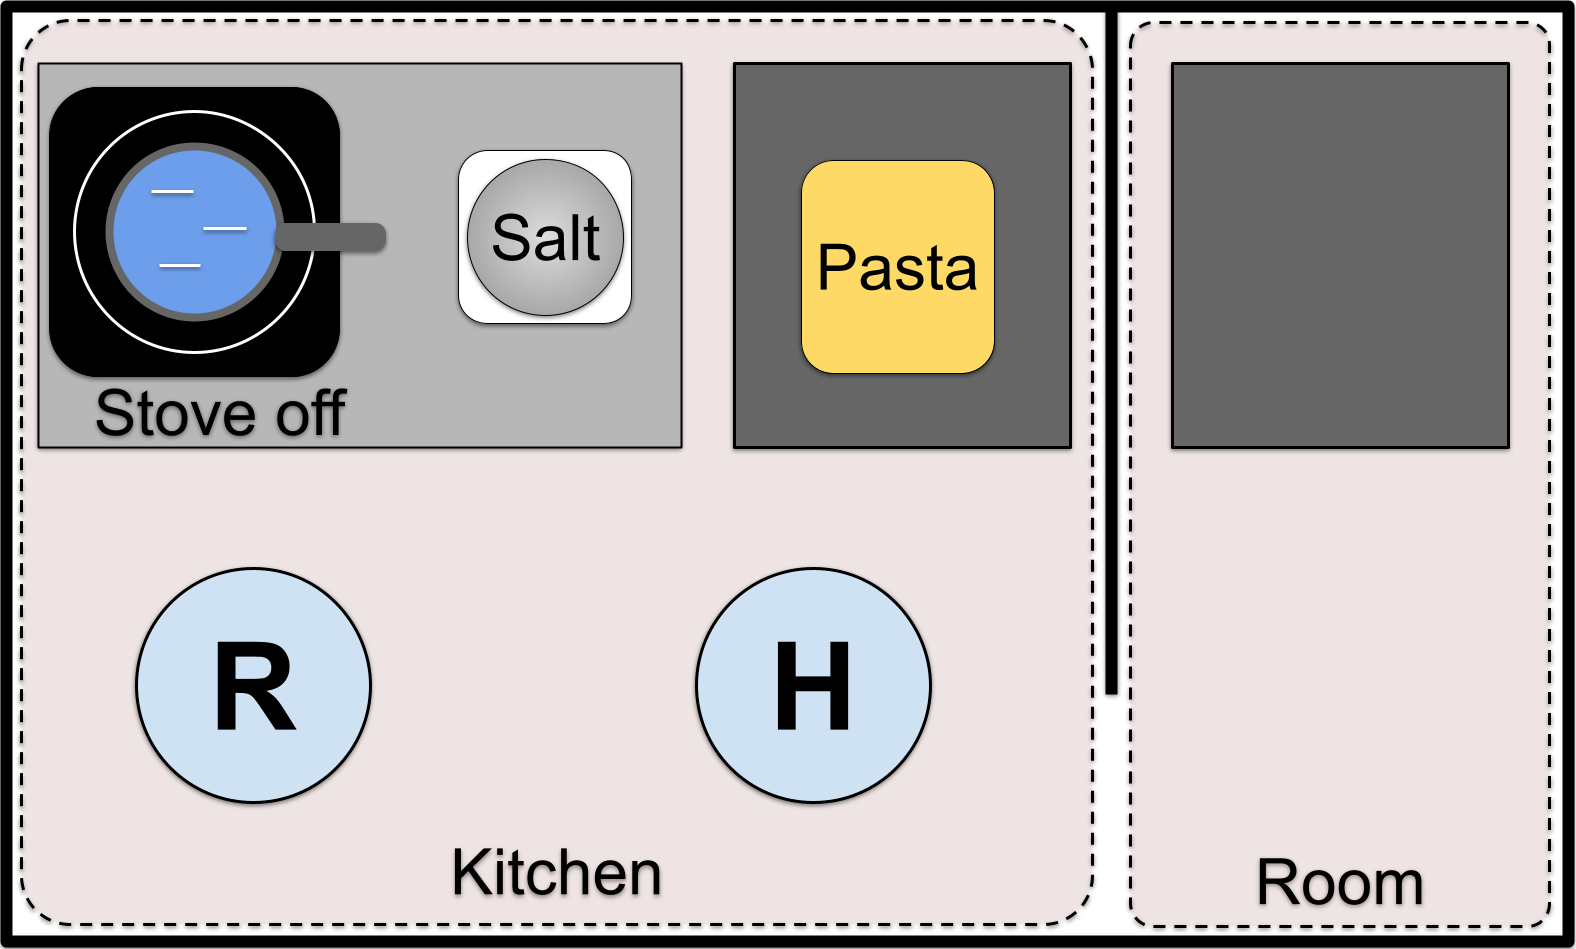
\includegraphics[width=0.8\linewidth]{figures/scene.png}
    \caption{Scene cooking}
    \label{fig:scene}
\end{figure}

Task description in HTN depicted in Fig.~\ref{fig:htn}

\begin{figure*}
    \centering
    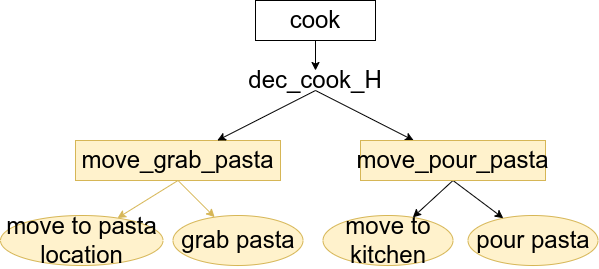
\includegraphics[width=0.4\linewidth]{figures/htn_human.png}
    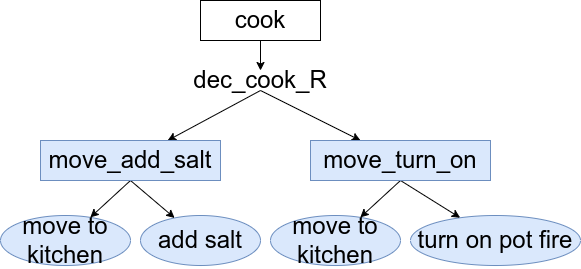
\includegraphics[width=0.4\linewidth]{figures/htn_robot.png}
    \caption{HTN, cook task description. Additional methods without the move action are not represented corresponding to when the agent is already at the right location.}
    \label{fig:htn}
\end{figure*}



\begin{figure*}
    \centering
    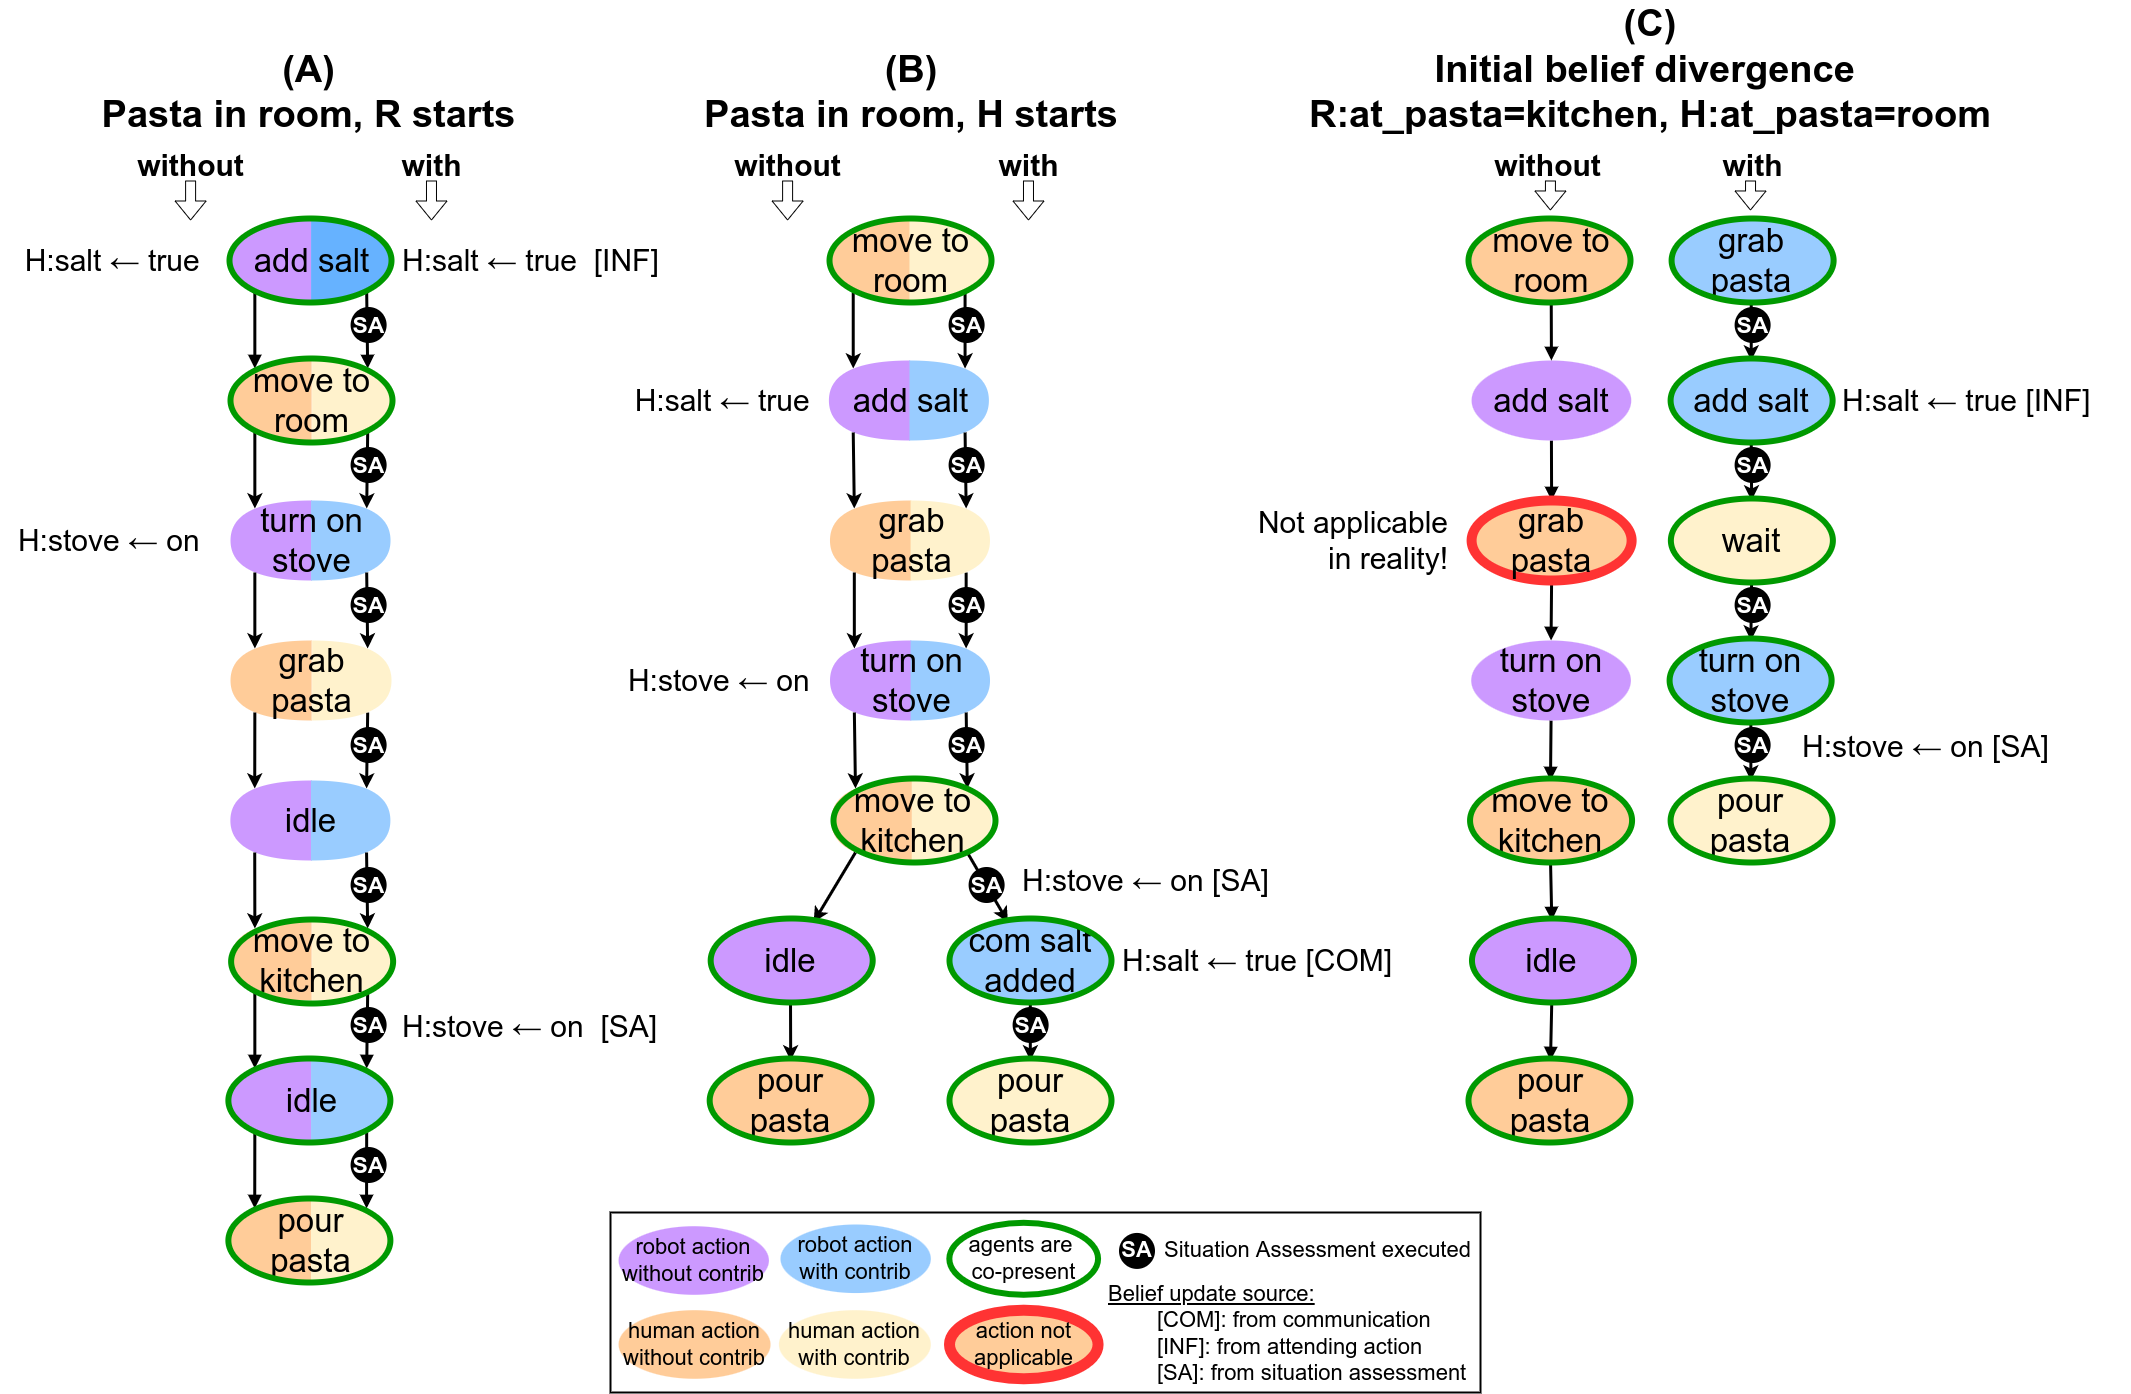
\includegraphics[width=\linewidth]{figures/example_cook.png}
    \caption{Caption}
    \label{fig:scenarios}
\end{figure*}


\subsection{Scenarios detailed}

In this section we focus on the plans obtained with and without our contribution in three different situations. First, both the human and the robot are initially in the kitchen, but the pasta is in the other room, thus the human will have to leave the kitchen. We consider first the case where the robot starts (A) and then when the human starts (B). The third situation includes an initial belief divergence. This time the pasta is already in the kitchen (robot could have brought them before the human arrives) but the human thinks they are still in the other room (C).  

For each situation (A,B,C), Fig.~\ref{fig:scenarios} depicts the plan computed and the updates of the human beliefs, both with (right side) and without (left side) the contribution. For legibility purposes when the actions computed are the same with and without the contribution they are merged.

% 72
\textbf{Scenario (A):} The plans obtained with and without the contribution are the same, however it's interesting to notice that the human beliefs are updated in the same way. In this scenario the human will not observe the "turn on pot fire" action of the robot. Without the contribution the agents are omniscient, so the human instantly knows about the effects of the robot action even being in the same room. With the contribution, we plan that the human will not observe the robot action thus their beliefs isn't updated. However, we predict that when coming back in the kitchen the human will assess the effects of the robot action and update their beliefs.

%73
\textbf{Scenario (B):} This time the human directly leaves the kitchen and will not attend both robot actions which will make the two plans differ. The plan obtained without the contribution is very similar to the (A) one. Before coming back, the human already knew about the salt and the fire. With the contribution, since we plan that the human will not be in the same place their beliefs isn't updated after each the robot action. When the human comes back in the kitchen they will assess the situation and notice that the fire is on. However, the "salt\_added" state-variable is only inferable, not observable, thus we predict that the human will not know about the salt even when back in the kitchen. Then, this belief divergence is detected as relevant since it has on influence on the human plan (they might add salt again in the pot). Thus, we decide to insert a communication action to correct the divergence and remove the ambiguity about the salt.

% 9
\textbf{Scenario (C):} Now the human thinks the pasta is in the other room, but the robot actually brought it to the kitchen before the human arrives. Without the contribution human next action are estimated using their beliefs ($\beliefs_\human$) so the human will move to the other room and try to grab the pasta. Since there is no pasta in the other room the grab action will fail with the ground truth (but not with $\beliefs_\human$), which makes the plan not valid. With the contribution, we rely on the fact that the human will update their beliefs themselves by assessing the situation and see that the pasta is already in the kitchen. Thus, no communication is needed.

\subsection{Quantitative}

We ran the planner, both with and without the contribution, on every possible initial state of the pasta cooking problem. The table below shows the success rate of the planner with the contribution (S w/) and without (S w/o). Without the contribution a planning failure can occur in two cases. First, if a human estimated action is not applicable (NA) in reality  or if an inactivity deadlock (IDL) has been reached, i.e. if there is a succession of at least four WAIT or IDLE actions. The ratio of failed planning due to non-applicable human action and due to inactivity deadlocks are given in the table as well.

\begin{tabular}{|c|c|c|c|c|}
    \hline
    \textbf{Problem} & \textbf{S w/} & \textbf{S w/o} & \textbf{NA} & \textbf{IDL}\\
    \hline
    Pasta cooking & 100\% & 25.7\% & 70.5\% & 29.5\%\\
    \hline
    Other & -\% & -\% & -\% & -\%\\
    \hline 
\end{tabular}

With the contribution the planner always find a valid plan that may include communication. When there are no initial belief divergence the planner without the contribution always finds a valid plan. However, the plan generated will always the agents as omniscient which may later lead to ambiguities when executing the plan in real life. Most of the scenarios that include belief divergence leads to non-valid plans without the contribution. Inactivity deadlocks occur when the human thinks the stove is off or that there is no salt, although it's already done, the robot will never do the corresponding actions again and the human beliefs will never be updated. Hence, the precondition of the "pour pasta" action will never be met.

% \begin{itemize}
%     \item w/o always working when there is no belief divergence initially. However, the plan generated will always the agents as omniscient which may later lead to ambiguities when executing the plan in real life. 
%     \item belief divergence on pasta location, R:at\_pasta=room H:at\_pasta=kitchen. Without: H try to grab pasta in kitchen but action not applicable in reality. With: Robot com to warn H that pasta are in room. Actually, H will be able to see that the pasta are not in the kitchen, they cannot see where it is but at least it's not in the kitchen, where they thought it was. We currently not handle explicit assessing of not knowing (assessing that the pasta are not here). However our planner still handles the cases because this divergence (here ambiguity) will affect the human plan thus it is considered as relevant, as a consequence R will communication to align $\beliefs_\human$ and remove the ambiguity.
%     \item div on pasta loc always leads to failure without (not app)
%     \item div on pot fire leads to failure (not applicable reality) only if there is no div on pasta loc (otherwise fails before due to pasta div) and if human tries to pour pasta before robot actually turns on fire. If R turn on fire before, it's not applicable with $\beliefs_\human$ but fixes the div.
%     \item failure inactivity deadlock without if H div on pot\_fire or salt = false although it's already done, thus the robot will never do them again and deadlock occurs
% \end{itemize}

\subsection{Interesting case}

An interesting case to focus on is a scenario close to (C) with a belief divergence on the pasta location. Both agents are in the kitchen and the pasta is in the other room, but the human thinks the pasta is in the kitchen. Without the contribution we estimate that the human will try to grab pasta in the kitchen which will fails in real life. [...] 



\section{Discussion}
% how do the results fill the gap ?

Point out ambiguities (created both by the lack of situation assessment and belief alignment) in the plans without contribution. Then, explain how we removed them. 

\section{Conclusion}
% what does this mean for us going forward ?

FUTURE WORK:
\begin{itemize}
    \item A more elaborated formula for observability than co-presence. Using geometrical reasoning with a physic simulator.
    \item Use an entity-based world description to be able to automatically update the $\loc{\fluent{\worldstate}{}{}{}}$.
    \item A more complex reasoning to decide where to insert the communication action in the plan.
\end{itemize}

\bibliography{bib.bib}

\end{document}
